%    DD-ERS.tex  (use only for JWST Director's Discretionary Early Release Science proposals)
%
%
%
%    JAMES WEBB SPACE TELESCOPE 
%    OBSERVING PROPOSAL TEMPLATE 
%    FOR CYCLE 1 DD-ERS (2017)
%
%    Version 1.0 May 2017.
%
%    Guidelines and assistance
%    =========================
%     Cycle 1 Announcement Web Page:
%
%         https://jwst-docs.stsci.edu/display/JSP/JWST+Cycle+1+Proposal+Opportunities
%
%    Please contact the JWST Help Desk if you need assistance with any
%    aspect of your proposal:
%    	    http://jwsthelp.stsci.edu
%
%
%
%%%%%%%%%%%%%%%%%%%%%%%%%%%%%%%%%%%%%%%%%%%%%%%%%%%%%%%%%%%%%%%%%%%%%%%%%%%

% The template begins here. Please do not modify the font size from 12 point.

\documentclass[12pt]{article}
\usepackage{jwstproposaltemplate,natbib,graphicx}
\usepackage{wrapfig}
\setcitestyle{aysep={}}
\usepackage{color}
\usepackage[utf8]{inputenc}
\bibliographystyle{apj}

\newcommand{\apj}{ApJ}
\newcommand{\apjl}{ApJL}
\newcommand{\apjs}{ApJSS}
\newcommand{\aap}{A\&A}
\newcommand{\aj}{AJ}
\newcommand{\mnras}{MNRAS}
\newcommand{\araa}{ARA\&A}
\newcommand{\pasp}{PASP}
\newcommand{\pasj}{PASJ}
\newcommand{\nat}{Nature}

% LKH
\def\myitem{\par\hang\textindent }
\newenvironment{parhang}{\hangafter=1\hangindent=10pt}{\par}

\begin{document}

%   1. RATIONALE FOR DD ERS Program
%       (see https://jwst-docs.stsci.edu/display/JSP/JWST+DD+ERS+Proposal+Preparation)
%
%
\rationaletime          % Do not delete this command.
% Enter your rationale for selection as a DD ERS program.

% Explain how the proposal will support community preparations for Cycle 2 observations. Describe the anticipated interest in, and use of, the data and science-enabling products developed by the team. Describe how the proposal will serve as a pathfinder for science investigations. 
\vspace{-0.1in}
\noindent {\bf Overview:} 
Nearby galaxies are critical to understanding galaxy evolution. Only there can observations directly resolve the vicinity of active nuclei, individual star-forming clouds and star clusters, while still covering a full galactic disk. This comprehensive view lets us connect the small-scale physics of the interstellar medium (ISM) and star formation (SF) to the disk-wide processes that drive galaxy evolution. JWST's angular resolution, sensitivity and coverage of the diagnostic-rich near- to mid-IR will revolutionize this field.

%Nearby galaxies connect what we learn from small-scale studies of the interstellar medium (ISM) and star formation (SF) in the Milky Way to the great diversity of galactic environments relevant for galaxy evolution. Only in nearby galaxies can observations directly resolve the central zones of active galaxies, individual star-forming clouds, and star clusters, while still being able to cover a full galactic disk. 
%We propose to observe the Whirlpool galaxy, M51, with a suite of JWST modes to study the link between small-scale phenomena observable in the Milky Way and large-scale characteristics that result from galaxy evolution. Only in nearby galaxies can both scales be studied in the same system, by directly resolving the central zones of active galaxies, individual star-forming clouds in the interstellar medium (ISM), and star clusters, while also covering a full galactic disk.

Over JWST's lifetime, the nearby galaxy community will propose many observations in a wide array of modes. While observing nearby galaxies may seem straightforward, their large angular extent, high dynamic range in surface brightness, and widespread extended emission present unique challenges. To prepare the community to address those challenges, {\em we propose to obtain a set of observations with NIRCam, NIRSpec and MIRI towards the nearby galaxy M51.} We have designed an efficient, multi-mode observing program that will allow the community to prototype critical science investigations and let us produce a set of Science Enabling Products crucial for galaxy research and beyond

M51 is the natural choice for a representative nearby galaxy. Because of its environmental richness, it has been extensively observed by facilities from X-ray through radio wavelengths. M51 hosts a Seyfert~2 AGN \citep{ho1997} which shows evidence for a jet interacting with the surrounding ISM \citep{querejeta2016} and a strong two-arm spiral  featuring deep dust lanes and feathers extending into the interarm regions \citep{lavigne2006}. At M51's distance of 8.6~Mpc \citep{mcquinn2016}, JWST's resolution samples the 3--30~pc scales of individual stellar clusters, star-forming regions, and molecular clouds. {\em Over its lifetime, JWST will conduct the types of observations we propose for M51 many times over for nearby galaxies.} Because of M51's broad ancillary database, it can serve to prototype many of these potential studies. 

Beyond preparing our community for future JWST observations, the program will address critical questions on the cycle of dust, gas, SF and feedback in galaxies, specifically: 
\vspace{-0.25in}
%\vspace{-1.5\baselineskip}
\begin{enumerate}
    %\itemsep0.1em 
    \item What sets the evolutionary timescale of individual star-forming molecular clouds?\vspace{-0.1in}
    \item How much dust is produced by evolved stars at solar metallicities?\vspace{-0.1in}
    \item How do small carbonaceous dust grains evolve in different galactic environments?\vspace{-0.1in}
    \item How does an AGN impact the ISM near galaxy centers, radiatively and mechanically?\vspace{-0.1in}
\end{enumerate}
%\end{itemize}

\vspace{0.05in}

\noindent Building the dataset to address these key topics involves imaging the main star-forming body of M51 in several photometric bands with NIRCam and MIRI, accompanied by targeted spectroscopy of the nucleus and a spiral arm with the NIRSpec and MIRI IFUs. Table~\ref{tab:overview} provides an overview of our proposed observations, science goals and science enabling products.

\begin{figure}
% \plotone{summary_figure}
 \includegraphics[width=6.5in]{summary_figure_DADv6.pdf} 
 %\caption{Caption here.}
\label{fig:overview}
\vspace{-0.3in}
\end{figure}


\begin{table}[htp]
\scriptsize
\caption{Overview of M51 Treasury Observations, Science Goals \& Science Enabling Products}
\begin{center}
\vspace{-0.2in}
\begin{tabular}{|l|l|l|l|l|}
\hline
Observation & Primary Science Goals & Additional Science Goals & Science Enabling Products & Lead\\
\hline
{\bf NIRCam mosaic} & 1.\ Life Cycle of SF Regions & Embedded Clusters & \#2 Cont. Subtr. Recipes & Bolatto\\
---F164N/F162M, & 2.\ Dust Production & Improve SFR Tracers & \#3 Convolution Kernels & Sandstrom \\
~~~F212N/F182M, & 3.\ Dust Evolution &  & \#4 Point Source Catalogs & Boyer \\
~~~F335M/F360M, & &  &  & \\
~~~F405N/F430M & & & &\\
\hline
{\bf MIRI mosaic} & 1.\ Life Cycle of SF Regions & Improve SFR Tracers & \#3 Convolution Kernels & Sandstrom \\
---F1000W, F1130W, & 2.\ Dust Production & 
% LKH edit propose to eliminate this additional science goal, difficult to explain and space limited Silicate Absorption 
& \#4 Point Source Catalogs & Boyer\\
~~~F2100W & 3.\ Dust Evolution & &  & \\
\hline
{\bf NIRSpec IFU} & 3.\ Dust Evolution & Metallicity Diagnostics & \#1 Spectral Templates & Dale\\
---R$\sim$1000 0.97--5.27\micron & 4.\ AGN Zone of Influence & H$_2$ Shock Heating & \#2 Cont. Subtr. Recipes & Bolatto\\
~~~~~~Nucleus Region &  & Wolf Rayet Signatures & \#3 Convolution Kernels & Sandstrom\\
---Prism 0.6--5.3\micron  & & & \#5 IFU Cal. Tests & Gordon\\
~~~~~~Arm Region & & & \#6 PAHFIT Extension & Smith\\
\hline
{\bf MIRI IFU} & 3.\ Dust Evolution  & Metallicity Diagnostics & \#1 Spectral Templates & Dale\\
---R$\sim$3000 4.9--28.8\micron & 4.\ AGN Zone of Influence & H$_2$ Shock Heating & \#3 Convolution Kernels & Sandstrom\\
~~~~~~Arm \& Nucleus & & Extragalactic C$_{60}$ & \#5 IFU Cal Tests & Gordon\\
---Simultaneous Imaging & & H$_2$ tracing CO-Dark gas & \#6 PAHFIT Extension & Smith\\
~~~~~~F2550W & &  & & \\
\hline
{\bf NIRCam Parallel} & & tRGB Population & \#4 Point Source Catalogs & Boyer\\
--F150W/F277W  & & Stellar Halo &  & \\
{\bf NIRISS Parallel} & & &  &  \\
--F090W/F150W/F200W & & & & \\
\hline
\end{tabular}\vspace{-0.3in}
\end{center}\label{tab:overview}
\end{table}%

%\vspace{0.1in}
\medskip
\noindent {\bf Science Enabling Products:} Beyond the JWST observations, our team will develop a suite of tools and documentation for the community that address key steps in the path from observation planning through processed data to science. 
% LKH edit for brevity The necessity of such tools and documentation is already evident from the preparation for this proposal and from the past experience of our team in a wide variety of nearby galaxy surveys.  
These include:

\vspace{0.05in}

\noindent {\bf (\#1) Near- to Mid-IR Spectral Templates:} JWST will enable near- through mid-IR spectral mapping with the resolution to separate molecular clouds and PDRs from H{\small II} regions and diffuse interarm material.  Spectroscopy from the ground has covered parts of the near-IR spectrum but over limited areas.  {\em Spitzer} performed extensive spectral mapping in the mid-IR but at $\sim$100~pc resolution. JWST's angular and spectral resolution plus wavelength coverage is such a dramatic leap beyond previous facilities that predicting necessary exposures, appropriate filter combinations, grism choices and more are challenging tasks for proposers. In the current JWST ETC, template options are limited to low spectral resolution galaxy-integrated measurements from  \citet{brown2014}. For that reason, one of our initial Science Enabling Products will be the delivery of near- through mid-IR spectral templates derived from our NIRSpec and MIRI IFU observations (which each cover $\sim$500$\times$125~pc over multiple environments).  We will create templates for resolved molecular regions/PDRs, H{\small II} regions, diffuse interarm emission (with stacking if needed), and the central AGN and jet.  We will work with STScI to incorporate these into the ETC for Cycle~2 proposers to use for observation planning. Later deliveries will include tools so observers can generate their own custom templates from the full coverage, resolution-matched, spectrally-stitched cubes. 

\vspace{0.05in}

\noindent {\bf (\#2) Continuum Subtraction Recipes:} Because of the small field of view of JWST's spectroscopic instruments, narrow and medium band imaging that isolates spectral lines will be a critical mode of JWST observing in nearby galaxies, where both high spatial resolution and wide area mapping are needed. For continuum removal and estimating exposure times, proposers need information on various medium band options and scaling factors. We will provide the community with documentation, code and examples of continuum removal using our NIRSpec, NIRCam and MIRI spectroscopy and imaging. We will use the spectral templates {\bf (\#1)} to predict scaling factors for all combinations of narrow and medium bands for NIRCam as well as medium band combinations in MIRI to isolate PAH features.  Those predictions will be tested on our NIRCam and MIRI images by comparing directly with the known line intensities from spectral mapping.  We will assess the quality of continuum removal across the galaxy and provide tutorials for applying it to future observations.  The initial NIRCam and MIRI recipes plus tests will be an early deliverable (prior to the Cycle~2 deadline).  In the longer term we will investigate optimizing combinations of multiple medium bands as well as spatially dependent recipes that vary across the galaxy.

%\vspace{0.05in}

%\noindent {\bf (\#3) Mosaic Documentation:} Mosaicking will be a critical observing mode for nearby galaxies. 
% LKH edit
%We will provide and test algorithms for background level matching and image alignment beyond what is routinely performed in the pipeline.

\vspace{0.05in} 

\noindent {\bf (\#3) Convolution Kernels and Routines:}  Over the wide wavelength coverage of JWST, the PSF width will vary by more than an order of magnitude and change shape from instrument to instrument. This makes PSF matching critical for comparing resolved emission across different instruments and spectral regimes. To enable this key step, we will generate a library of convolution kernels that match JWST observations across wavelength and instrument, including for IFU spectral maps.  Members of our team generated kernels that have been widely used to analyze {\em Spitzer} and {\em Herschel} observations \citep{gordon2008,sandstrom2009,aniano2011}. We will also provide kernels that match JWST observations to PSFs from other facilities (e.g., {\em Spitzer}).  Our team will provide versions of these kernels based on the theoretical PSFs early in 2019, update those kernels with observed PSFs, and test the resulting convolution on our M51 dataset.  We will also create open-source Python code to perform convolutions using the kernels.

\vspace{0.05in} 

\noindent {\bf (\#4) Point Source Photometry Catalogs \& Documentation:} JWST's sensitivity and angular resolution make luminous stars, particularly the Asymptotic Giant Branch (AGB) and red giant/supergiant stars, observable in galaxies out to $\sim$10~Mpc, even in crowded disks like that of M51.  Resolved stars will also be frequently observed in parallel observations, typically sampling galaxy halos. Detecting resolved stars in nearby galaxies, even serendipitously, will thus be a routine occurrence for JWST observers.  To prepare the community for  such observations, we will create software tools and demonstrate photometry in both M51's disk using our NIRCam and MIRI imaging, and in the sparse outer halo as observed in parallel with NIRISS/NIRCam.  Documentation and tutorials will be provided to the community, in addition to the results of artificial star tests to characterize the photometric uncertainty and completeness limits of the catalogs.

\vspace{0.05in} 

\noindent {\bf (\#5) IFU Calibration Tests:} Bright, extended nearby galaxies pose some challenges for IFU observations with JWST. For NIRSpec, leakage through faulty MSA slits will contaminate the observations.  When those slits sit on top of a bright galaxy like M51, contamination will be a major concern.  The conservative approach is to obtain ``leakcal'' observations with the same configuration for each observation, doubling the needed time investment.  For MIRI, extended sources make it impossible to use nodding to remove the sky and telescope thermal backgrounds and spectral fringing.  Therefore, an ``off'' position will be required, at large angular separation. The performance of ``off'' observations is not well known as a function of time difference from when the target observations are taken.  We will obtain a conservative set of calibrations for our IFU spectroscopy including NIRSpec ``leakcals'' at every position, dither, and grating setting and MIRI ``offs'' both before and after our science observations. We will assess the performance of the complete calibration set, and the consequences of omitting different aspects (e.g., obtaining a MIRI ``off'' 10 hours after the target or one ``leakcal'' per mosaic position) by dropping parts of the calibration set in the processing. This information will aid community planning for efficient JWST IFU observations in extended objects and these tests will be in our earliest set of deliverables.

\vspace{0.05in} 

\noindent {\bf (\#6) Updating PAHFIT for the JWST era:}  Galaxy mid-infrared spectra are rich with diagnostics of molecular and ionized gas and dust grains, all set against a variable blend of starlight, hot grain emission, and other continuum sources, attenuated by opacity from ices and silicates.  Disentangling this complicated spectral region requires physically motivated and empirically validated modeling.  PAHFIT, developed for {\em Spitzer}/IRS spectroscopy, is the preeminent tool for the decomposition of mid-IR spectra of galaxies and other sources \citep{smith2007}.  Updating PAHFIT for the JWST era will be critical to fully exploit the diagnostic potential offered by the combined NIRSpec/MIRI IFUs.  We will adapt PAHFIT to {\em i}) treat the high and variable spectral resolution, including newly resolved PAH sub-features, {\em ii}) extend wavelength coverage down to 2\micron\ with preliminary pre-launch input from an ongoing {\em Akari}--{\em Spitzer} cross-archival study, and {\em iii}) introduce updated extinction models for both ices and silicates.  Early M51 spectroscopy will be a crucial first step in bringing the power of spectral decomposition to the JWST community.


%Concerning fringes, I think the best we could do is to assess the wuality of the fringes correction in the pipeline. Impact of the residuals, most affected wavelengths, impact in the SNR of faint emmission or absorption lines, whether residuals can be mistaken for lines etc. Just informing the community and giving feedback to the pipeline.

%To illustrate their importance for nearby galaxy observations, we describe the path from planning through science for each of our four key science goals, and highlight the need for the following products: {\bf (\#1)} near- to mid-IR spectral templates, {\bf (\#2)} continuum removal recipes for narrow and medium band filters to create line maps, {\bf (\#3)} documentation of mosaicking performance and efficiency, {\bf (\#4)} convolution kernels and programs to match point-spread functions across JWST's wavelength range, {\bf (\#5)} documentation, catalogs and artificial star tests for point source photometry in crowded fields, {\bf (\#6)} documentation of the performance of ``off'' and leakage calibrations for IFU spectroscopy towards extended, high contrast objects, and {\bf (\#7)} extension of the PAHFIT spectral decomposition model to target JWST observations.

%\vspace{0.1in}

%\noindent {\bf Science Goal 1.~Life Cycle of Star-Forming Regions:} This investigation relies on the statistical constraints provided by galaxy-wide, $\sim$10 pc scale observations of emission lines from gas, SF (ionized gas, star clusters), and feedback (shocked gas, supernovae).  Wide-area coverage in emission line diagnostics can be obtained using JWST's narrow and medium band imaging modes.  For planning such observations, a key resource that is not yet easily available is near- through mid-IR spectral templates for different galactic environments {\bf (\#1)} that facilitate planning narrow band imaging.  To create line maps, we must remove continuum from the narrow band and we will investigate the optimal method and choice of bands for this process using the spectral mapping {\bf (\#2)}.  Wide-area maps of nearby galaxies will involve mosaicking to cover large regions {\bf (\#3)}, which we will demonstrate and document in multiple filters. Lastly, a key step for multiwavelength comparisons for extended sources will be convolution to matched point spread functions {\bf (\#4)}.  

%\vspace{0.05in}

%\noindent {\bf Science Goal 2.~Dust Production by Evolved Stars:} JWST imaging will reveal the current rate of dust production in nearby galaxies by detecting dusty evolved stars. Our NIRCam and MIRI imaging will isolate distinct spectral features in AGB star SEDs. For these observations, it will be necessary to extract point source photometry from the crowded field of a nearby galaxy.  Our team will generate documentation, point source catalogs and artificial star tests {\bf (\#5)} demonstrating the feasibility of such observations and providing technical guidance on point source photometry. 

%\vspace{0.05in}

%\noindent {\bf Science Goal 3.~Evolution of PAHs:} JWST enables the first detailed studies of the 3.3/3.4\micron\ PAH features (NIRCam imaging, NIRSpec spectroscopy) in galaxies, as well as high spatial resolution diagnostics of the full PAH spectrum (MIRI imaging and spectroscopy). We will use NIRCam and MIRI imaging {\bf (\#1, \#2)} as well as NIRSpec and MIRI IFU spectroscopy to reveal key aspects of the PAH lifecycle in M51. Our program includes a conservative set of IFU calibrations (e.g., ``off'' observations and leak calibrations) which we will use to document for the community the necessity and efficacy of such calibrations {\bf (\#6)}.  For analysis of NIRSpec and MIRI spectroscopy of PAHs, we will extend the Spitzer-based PAHFIT spectral fitting routine \citep{smith2007} to incorporate features in the near-IR and adapt it to JWST's spectral resolution {\bf (\#7)}.

%\vspace{0.05in}

%\noindent {\bf Science Goal 4.~Resolving the AGN's Zone of Influence:} NIRSpec and MIRI IFU observations will provide resolved diagnostics of the radiative and mechanical feedback from M51's AGN.  Future studies of nearby AGN will benefit from the spectral templates we generate from our AGN and H{\small II} region spectral datasets {\bf (\#1)}, our investigation of necessary IFU calibrations {\bf (\#6)}, convolution kernels to extract matched spectra from the IFU datacubes {\bf (\#4)}, and the PAHFIT extensions to analyze the spectral mapping data {\bf (\#7)}.

%\vspace{0.1in}

%\noindent These science enabling products will streamline the path from JWST proposal to science-ready data for our community.

\vspace{0.1in}

%\noindent {\bf The M51 ERS Team:} We have assembled a diverse, international team of 55 researchers spanning a range of scientific interests.  Our team includes the PIs of several large surveys of M51 who have made or will make their data public: PAWS CO (Schinnerer), the SOFIA C$^{+}$ survey (Pineda, Stutzki), multi-epoch HST imaging (Conroy), extensive Spitzer spectral mapping (Kennicutt), and more. To achieve our science goals and demonstrate multiple nearby galaxy JWST observing modes, we have optimized our strategy to improve the observational efficiency for relatively short exposure times for nearby galaxies and identified synergies between various science cases, e.g., AGB diagnostics and NIRCam imaging. Our team will rapidly share the knowledge we gain with the extragalactic community through Science Enabling Products, data products, and documentation on a dedicated website. As part of our ERS program, M51's ancillary observations, many of which were collected by our team, will be astrometrically aligned and placed on a dedicated website, enabling a vast multiwavelength synergy with JWST. 

\noindent {\bf The M51 Treasury Team:} We have assembled an international team of 54 researchers whose expertise spans the breadth of science that JWST will do in nearby galaxies: from studying the $\sim$pc vicinity of AGN to the substructure in the stellar halo. The process of bringing together such diverse expertise has let us create an observing program that efficiently captures a dataset useful for almost any nearby galaxy researcher. Our team is well prepared to create and deliver the Science Enabling Products described above, as demonstrated by our roles in generating such products for previous missions \citep{dale2006,smith2007,gordon2008,aniano2011,boyer2013}.  We will rapidly share our knowledge with the community through science and observation planning telecons and a dedicated website where we will post updates and host a repository of M51's ancillary observations, many of which were collected by our team members.

%%%%%%%%%%%%%%%%%%%%%%%%%%%%%%%%%%%%%%%%%%%%%%%%%%%%%%%%%%%%%%%%%%%%%%%%%%%

%   2. SCIENTIFIC JUSTIFICATION
%       (see https://jwst-docs.stsci.edu/display/JSP/JWST+DD+ERS+Proposal+Preparation)
%
% Describe the scientific objectives supported by the proposed DD ERS observations and their overall importance to astronomy.  Describe the selected aspects of the science to be directly funded by the DD ERS program.  Discuss how the proposed observations support investigations beyond the immediate scientific objectives. 

\vspace{-0.5\baselineskip}

\justification          % Do not delete this command.
% Enter your scientific justification here. 
\vspace{-0.1in}
\noindent {\bf Science Goal 1.~The Life-Cycle of Star-Forming Regions:} Stars and clusters form out of molecular gas and then exert strong feedback on their parent clouds. A major goal of current ISM and SF studies is to understand how this violent life cycle produces the observed large scale relationship between gas and star formation \citep[e.g.,][]{kennicutt2012}. This can best be achieved via high resolution observations of nearby galaxies that resolve tracers of feedback, the ISM, and SF cloud-by-cloud over a large, well-characterized environment.

%We need to understand the mechanisms regulating the life cycle of a molecular cloud (e.g., feedback, large-scale dynamics, other factors), and the dominant feedback process for each evolutionary stage \citep[e.g.,][]{lopez2011,lopez2014}.

%How this feedback drives the relationship between gas and SF \citep[e.g.,][]{kennicutt2012} can best be understood from high resolution observations of nearby galaxies. We need to understand the mechanisms regulating the life cycle of a molecular cloud (e.g., feedback, large-scale dynamics, other factors), and the dominant feedback process for each evolutionary stage \citep[e.g.,][]{lopez2011,lopez2014}.

%Answers can be gained from population statistics, pairing region-by-region SF, molecular gas and feedback tracers across the well-characterized environment of a nearby galaxy. 

JWST is ideal for such studies. Pairing high resolution with IR diagnostics will allow us to measure the physical state of the gas, trace otherwise invisible SF, and identify feedback signatures cloud-by-cloud. Our observations of M51 will yield galaxy-wide maps of hot dust, ionized gas, radiative-phase supernova (SN) remnants and shocks via [Fe{\small II}] \citep{alonso-herrero2003} and vibrationally-excited H$_2$. We will compare these signatures of feedback and SF to the properties of the 1,500 molecular clouds already known and characterized in the inner 9$\times$7~kpc$^{2}$ of M51 \citep{colombo2014}. We will assign each individual cloud an evolutionary state (star-forming, quiescent, being destroyed), which is impossible to do at {\em Spitzer}'s resolution outside the Local Group. From the population statistics, we will model the life cycle and destruction mechanism for molecular clouds \citep[e.g.,][]{corbelli2017}.

%. The timescales inferred from statistical modeling of the populations will help constrain which mechanisms destroy the clouds \citep[e.g.,][]{kruijssen2014,corbelli2017}.

%JWST is ideal for such studies. Pairing high resolution with IR diagnostics will allow us to diagnose the physical state of the gas, trace otherwise invisible SF, and identify feedback signatures cloud-by-cloud. Our observations of M51 will yield galaxy-wide maps of hot dust, ionized gas, radiative-phase supernova (SN) remnants and shocks via [Fe{\small II}] \citep{alonso-herrero2003}, and vibrationally excited H2 via the 1-0S(1) line. These maps can be compared to detailed molecular cloud morphology and kinematics in the inner 9$\times$7~kpc$^{2}$ of M51 where $\sim$1500 clouds have been characterized \citep{schinnerer2013,schinnerer2017,meidt2015}. JWST's $\sim$10s~pc resolution will allow us to assign each cloud an evolutionary state (star-forming, quiescent, being destroyed). The timescales inferred from statistical modeling of the populations will help constrain which mechanisms destroy the clouds \citep[e.g.,][]{kruijssen2014,corbelli2017}.

High resolution JWST observations of the 3--5\micron\ hot dust continuum and Br$\alpha$ will also reveal new heavily embedded young clusters and yield accurate dust extinctions (and thus better ages and masses) for already-known young clusters. Only the brightest deeply embedded clusters were found by {\em Spitzer} \citep[][]{elmegreen2014}. With much deeper observations and $>$10$\times$ better angular resolution ($<$0\farcs2), we will detect embedded clusters with masses as low as 3$\times$10$^3$ M$_{\odot}$, giving us a much more complete snapshot of this early, hidden phase of star formation. The abundance of young clusters in the arm vs.\ interarm regions will indicate the relative importance of two main star/cloud formation drivers---spiral shocks and self-gravitational clumping in the arms \citep{kim2002}---and measure the persistence of star formation downstream from the spiral arm \citep{koda2009}. 

%plus existing HST imaging \citep{chandar2016}) will yield accurate dust extinctions and thereby better constrain cluster ages and masses. 

%JWST will also reveal the youngest clusters, allowing us to establish the link between spiral arms and SF. A combination of by observing obscured star clusters in molecular clouds in the 3--5\micron\ hot dust continuum. JWST Br$\alpha$ plus HST imaging \citep{chandar2016} will yield accurate dust extinctions and thereby better constrain cluster ages and masses. Only the brightest of these clusters have been found so far using Spitzer 3.6\micron\ images \citep[2\arcsec\ resolution;][]{elmegreen2014}. With much deeper IR observations at $\sim$10$\times$ better angular resolution (0\farcs2), we will detect embedded clusters down to $3\times10^3$ M$_{\odot}$. The relative proportion of these clusters in 
% the arm/interarm regions will indicate the relative importance of two main cloud formation mechanisms: spiral shocks and self-gravitational clumping in the arms \citep{kim2002}. We will also search for embedded clusters in interarm clouds \citep{koda2009} to see how long star formation persists downstream. 

%JWST will also reveal the link between spiral arms and SF by observing the youngest massive stars and star clusters still highly obscured by their natal clouds. Only the brightest of these sources have been found so far using Spitzer 3.6\micron\ images (2\arcsec\ resolution; Elmegreen et al.\ 2014). With much deeper IR observations at $\sim$10$\times$ better angular resolution (0\farcs2), we will determine the environments of a large number of clusters. JWST's ability to trace molecular material using extinction maps will also allow us to test whether the interarm clouds are filaments aligned with the arm (related to spiral shocks), or spurs, feathers, and shells developing downstream from the arms, or clumps condensed by gravitational instability or due to agglomeration.
%Furthermore, we will see if these clouds, traced by A$_V$ maps and embedded sources, are still filaments aligned with the arms in the case of spiral arm shocks, or spurs, feathers, and shells that develop downstream from the arms, or clumps that condensed by gravitational instabilities or agglomerated in the shocks. 
% LKH edit
%We will also search for SF indicators in the interarm molecular clouds \citep{koda2009}. These observations will allow the first direct determination of the SF efficiency in the arm and interarm regions, which we will compare to models of SF triggered by spiral shocks and secondary processes.
%We will compare  star-formation efficiency in the arm/interarm regions through JWST SF indicators  (Br$\alpha$) and PAWS molecular cloud properties, and compare to models of SF triggered by spiral shocks and secondary processes.


% LKH edit \vspace{0.05in}
%\vspace{0.1\baselineskip}
\noindent \underline{Additional Science Goals \& Prototypes:}

% LKH edit save space 
%\begin{itemize}\vspace{-0.1in}
% does not work \begin{itemize}[leftmargin=*]
   %\vspace{-0.1in}
  %LKH edit this is redundant w.r.t. preceding paragraph. Tried to integrate in order to save space \item {\bf Embedded Clusters:} We will detect young embedded clusters via 3--5\micron\ hot dust continuum with NIRCam and NIRSpec. JWST Br$\alpha$ plus HST imaging \citep{chandar2016} will yield accurate dust extinctions and thereby more accurate cluster ages and masses. We will use the observed luminosity/mass function of embedded clusters to answer: What fraction of embedded clusters are missed by shorter wavelength surveys?  How long do clusters remain embedded?  
   %What fraction of stars form in clusters, and does this value approach 100\% during the youngest embedded phase?
   %\vspace{-0.1in}
   
    %\item 
    % LKH edit
    % \myitem
    \begin{parhang}
    \noindent
    $\bullet$~{\bf Improve SFR Tracers:} Combining JWST Br$\alpha$ with existing HST H$\alpha$, Pa$\alpha$, and Pa$\beta$, we will measure extinction towards H{\small II} regions, test empirical extinction estimators and proposed IR cirrus corrections, and calibrate alternative SFR indicators (e.g.\ 11.3\micron\ PAH).% \vspace{-0.1in}
    % observations diagnose ionizing photon absorption by dust
    \end{parhang}
   %\begin{itemize}\vspace{-0.1in}  
    %\item 
    \begin{parhang}
    \noindent
    $\bullet$~{\bf Tracing CO-Dark Gas with H$_{2}$:} We will combine the H$_2$ rotational and vibrational emission spectrum observed by JWST with existing CO, [C{\small II}] and dust maps to probe the mass and state of the CO-dark H$_2$ gas component \citep[e.g.,][]{togi2016}.
    \end{parhang}
        
    %\item 
    \begin{parhang}
    \noindent
    $\bullet$~{\bf Metallicity Diagnostics:} We will calibrate extinction- and temperature-insensitive metallicity diagnostics, using optical-mid-IR spectral coverage provided by LBT-MODS \citep{croxall2015}, NIRSpec, and MIRI towards the H{\small II} region in the spiral arm spectral strip. JWST's resolution will allow matched aperture extraction of the optical through mid-IR neon and sulfur lines and mid-IR H recombination lines. With matched Br$\alpha$, [Ne{\small II}]12.81\micron, and [Ne{\small III}]15.56\micron, H{\small II} region metallicities will be accurately determined.
    % LKH edit for brevity overcoming the major issues with previous studies of mid-IR metallicity diagnostics. %\vspace{-0.1in} Detection of [NeII]12.8um and [NeIII]15.6um, together with Br alpha, will provide an accurate determination of HII region metallicities, insensitive to temperature uncertainties and almost independent of extinction.
    \end{parhang}
%\item 
     \begin{parhang}
    \noindent
    $\bullet$~{\bf Wolf Rayet Signatures:} We will identify WR stars (3--5~Myr; $>$25$M_\odot$), if present, with NIRSpec spectra  covering multiple C{\small IV}, He{\small I} and He{\small II} emission lines \citep{pasquali2002,kanarek2017}. We will use them to independently determine cluster ages and study their role in driving feedback \citep[e.g.,][]{sokal2016}. 
    \end{parhang}
%\end{itemize}

\vspace{0.2\baselineskip}
\noindent {\bf Science Goal 2.\ Dust Production:} Stellar evolution models of cool evolved stars, including intermediate-mass AGB stars and massive red supergiants (RSGs), remain highly uncertain due to complex mixing, dredge up, and mass loss processes. Their short lifetimes also make them rare, resulting in few statistically robust samples, especially in the IR where their spectral energy distributions peak. Together with SN ejecta and grain growth in the interstellar medium, both AGB and RSG stars contribute to the dust budget \citep{matsuura2009,boyer2012,srinivasan2016}. Because of distance uncertainties in the Milky Way,  extragalactic surveys are critical for constraining models and understanding dust production from evolved stars in metal-rich environments. 
% LKH edit These stars (both AGB and RSG stars) contribute to a galaxy's dust budget, with other sources being condensation in supernova ejecta and growth in the interstellar medium (Matsuura et al.\ 2009; Boyer et al.\ 2012; Srinivasan et al.\ 2017).

%These stars are among the brightest objects in galaxies, contributing up to 70\% of the near-IR luminosity (Maraston et al.\ 2006; Melbourne et al.\ 2012), depending on the SF history. Models have few empirical constraints on their lifetimes and therefore luminosity contribution, leading to significant biases in the interpretation of galaxy spectra (Conroy et al.\ 2009; Girardi et al.\ 2013). Chemically, AGB stars are uniquely responsible for elements used to derive metal abundances of metal-poor stars and possible self-enrichment of multiple populations in globular clusters (Ventura et al.\ 2001; D'Antona et al.\ 2002), but the connection between initial stellar mass and chemical yields is not calibrated, especially at high metallicity (Karakas \& Lattanzio 2014). In addition, these stars (both AGB and RSG stars) are the only confirmed contributors to a galaxy's dust budget (alternatives being possible supernova dust or interstellar grain growth), and may in fact dominate the dust production (Matsuura et al.\ 2009; Boyer et al.\ 2012; Srinivasan et al.\ 2017).

JWST's angular resolution, sensitivity, and wavelength coverage will revolutionize our understanding of dust-producing evolved stars in nearby galaxies. Optical HST data from \citet{mcquinn2016} demonstrate that AGB and RSG stars are easily identified in the disk of M51, despite issues of crowding and confusion. In the near-IR, these stars are even brighter, ensuring detection with JWST. NIRCam imaging in F162M, F182M and F360M will sample the SED and key molecular features  (H$_2$O, CN, C$_2$, SiO, and HCN) essential for estimating the stellar mass and the strength of mixing processes in the atmosphere. This filter set also efficiently separates C-rich and O-rich AGB stars (see Figure~1). MIRI imaging will sample the circumstellar dust, revealing the dust mineralogy and production efficiency (F1000W and F1130W sample silicate features in O-rich AGB stars and F430M and F2100W sample the dust continuum). Together the NIRCam and MIRI observations will constrain the composition and dust production rate of all of M51's evolved stars.
%LKH edit: need longer wavelengths (25 um or more) to sample the "shoulder" usually attributed to MgS in these stars, see Messenger, Speck, Volk 2013, now in bibliography.
%F2500W samples MgS in C-rich AGB stars, 

% LKH edit \vspace{0.1in}
\vspace{0.2\baselineskip}
\noindent {\bf Science Goal 3.~The Evolution of PAHs:} Mid-IR emission from small dust grains provides a critical glimpse into the composition and properties of interstellar dust. Single photons can heat small grains to non-equilibrium temperatures, exciting internal vibrational modes that reveal their structure and composition. The mid-IR bands of PAHs are one of the most easily observable of these features. Roughly 5\% of all the non-primordial radiative energy emitted over the full history of the Universe has been channeled through PAHs, emerging either as mid-IR emission or photoelectrons \citep{dole2006,smith2007}. The PAH spectrum and photoelectric heating efficiency depend on the abundance, size, and charge of the PAHs---properties that have all been suggested to vary within galaxies \citep{bakes1994,weingartner2001,croxall2012}. JWST will dramatically advance characterization of PAHs with its high angular resolution and ability to cover the critical PAH 3.3\micron\ feature. This feature is dominated by the smallest, neutral PAHs that can survive in the ISM. Most longer wavelength PAH bands are formed from combinations of neutral and ionized PAHs across a range of sizes, and so have more limited diagnostic potential. However, the 11.3\micron\ feature is dominated by large neutral PAHs \citep{bauschlicher2008}; thus the ratio of the 3.3/11.3\micron\ features, both of which JWST can efficiently observe, provides the most unambiguous size diagnostic of the PAH population.

We will use the 3.3\micron\ spectral region, made newly accessible via JWST imaging and spectroscopy, to study the evolution of PAHs in M51. The NIRCam F335M and MIRI F1130W will let us create high resolution maps of the 3.3/11.3\micron\ ratio, revealing the PAH size distribution across the galaxy. With NIRSpec spectroscopy, the 3.3\micron\ region will reveal new diagnostics of PAH chemical structure: the 3.4\micron\ aliphatic feature traces linear carbon-chain vibrational modes that are highly diagnostic of the structural state of the smallest grains \citep{joblin1996}.  We will study variations of the 3.3/3.4\micron\ features across a spiral arm using the relative aliphatic content to infer grain growth and chemical alteration of PAHs in dense regions \citep[e.g.,][]{berne2009} as well as production of PAHs via shattering \citep{yamagishi2012}.  Previous facilities did not have the combined spectral coverage, sensitivity, and angular resolution required to investigate these PAH diagnostics in galaxies. 

%Our observations will provide the first glimpse of the diagnostic potential of the 3.3/3.4$\micron$ ratio within galaxies and what it may reveal about the life cycle of PAHs. 

%\vspace{0.1in}

\noindent \underline{Additional Science Goals \& Prototypes:}
%LKH edit for brevity \begin{itemize}\vspace{-0.1in}
% \item 

    \begin{parhang}
    \noindent
    %$\bullet$~{\bf Silicate Absorption:} We will use MIRI imaging to map silicate absorption across the galaxy, revealing dense dust concentrations that were unresolved by Spitzer in M51.  We will also measure ice extinction features, silicate crystallinity, and more from the NIRSpec and MIRI spectroscopy. 
    % LKH comment: how to map absorption from MIRI imaging is not clear, maybe eliminate for reasons of space?
    %\vspace{-0.1in}
     %\item
     \end{parhang}
     \begin{parhang}
     \noindent
    $\bullet$~{\bf Extragalactic C$_{60}$:} Buckminsterfullerene has been observed in a number of reflection and planetary nebulae, but has not yet been detected outside the Local Group.  JWST's sensitivity and the ability to isolate intense PDRs and stellar remnants at high angular resolution will give us the first opportunity to place strong limits on C$_{60}$ in M51.
    % LKH edit what is the wavelength of C$_{60}$?$
    \end{parhang}
    %\vspace{-0.1in}
    % \item 
    \begin{parhang}
    \noindent
    $\bullet$~{\bf H$_2$ Shock Heating:} Rotational H$_2$ lines are one of the major coolants of warm molecular gas above 100~K. %and thus provide direct constraints on the dominant excitation mechanisms and average physical conditions in the mixing zone between atomic and molecular gas. They are and are therefore sensitive to photoelectric heating via collisions, shocks, X-ray heating, and under specific circumstances direct UV excitation followed by fluorescence. 
    Their strength relative to PAH emission is now regularly used as a signpost of shocks. %, when the H$_2$/PAH luminosity ratio exceeds a certain threshold. They could thus become a useful tool to delineate regions where shocks are induced by non-circular motions or by supernovae, complementary to velocity measurements and other shock tracers.
    We will use the rotational excitation and PAH emission from MIRI spectroscopy to quantify densities and temperatures, diagnose shocks, and trace departures from ortho-para equilibrium tied to thermalization timescales of shocked gas. Such departures were found in some {\em Spitzer}/IRS pointings within M51 and other galaxies  \citep{roussel2007}, but  the coarse angular resolution and low sensitivity of those observations prevented the thorough analysis that will now be possible with MIRI.
    \end{parhang}
    %\vspace{-0.1in}
%\end{itemize}

\vspace{0.05in}

\noindent {\bf Science Goal~4. Resolving the AGN's Zone of Influence:} 
JWST observations will provide an unprecedented view of the interaction of AGN with their surrounding ISM by spatially resolving key mid-IR observables. Intense AGN radiation heats nearby dust up to sublimation temperatures, with the bulk of its emission emerging in the $\sim$3--20\micron\ range. This process potentially alters the dust size distribution from a standard ISM distribution to favor predominantly large grains  \citep[e.g.,][]{kishimoto2007,honig2017}. However, the role of the AGN in exciting and/or destroying the PAHs is still uncertain within $\sim100$~pc \citep{smith2007,jensen2017}.

The hard AGN radiation and the shocks created by outflows and jets are able to ionize and excite the ISM to levels far above that possible in H{\small II} regions.  JWST offers access to near- and mid-IR line diagnostics that can clearly trace the impact of the AGN  and shocks, and separate them from the effects of young stars  \citep{dale2004,dale2009,scharwachter2013,colina2015,smajic2015}. Nuclear pointings of the NIRSpec IFU will detect coronal lines such as [Si{\small VI}]1.963\micron\ and [Si{\small VII}]2.483\micron\ that probe the AGN ionizing spectrum, and lines such as [Fe{\small II}]1.644\micron\ that are known tracers of shocks.  Nuclear pointings of the MIRI IFU will access mid-IR AGN diagnostics, such as those based on the [Ne{\small V}]/[Ne{\small II}] ratio and PAH equivalent widths. Quantifying the AGN emission will lead to a robust determination of the local SFR to assess whether SF is locally suppressed or enhanced by AGN-related shocks  \citep{silk2013}. The spectroscopic observations with R$\sim$1000--3000 will resolve $v \sim$100~km/s and reveal the structure of molecular gas (H$_2$) and dust in the nuclear environment, as well as kinematically reconstruct the resolved outflow and allow us to directly connect the ionization and heating of the gas with the dynamics of the ISM.

In M51, observations from the JVLA (synchrotron), PdBI (CO), and HST (H$\alpha$ and [O{\small III}]5007) indicate the orientation of the AGN jet and the location of possible AGN impacted gas for purposes of orienting our spectral ``strip'' observations \citep{querejeta2016}.  


%\vspace{0.1in}

%\noindent \underline{Additional Science Goals:}
%\begin{itemize}\vspace{-0.1in}
%    \item {\bf Test AGN unification theory} via measuring nuclear silicate emission and/or absorption\vspace{-0.1in}
 %   \item {\bf Gas flow onto and from the AGN} reveal the structure of dense gas (e.g., H$_2$ lines) and dust emission in the nuclear environment (e.g., spirals as signs for inflows) and kinematically reconstruct the resolved outflow\vspace{-0.1in}
%    \item {\bf Jet/Disk Orientation} constrain relative orientation of the jet and accretion disk\vspace{-0.1in}
%\end{itemize}

%%%%%%%%%%%%%%%%%%%%%%%%%%%%%%%%%%%%%%%%%%%%%%%%%%%%%%%%%%%%%%%%%%%%%%%%%%%

%   3a. DESCRIPTION OF THE OBSERVATIONS
%       (see https://jwst-docs.stsci.edu/display/JSP/JWST+DD+ERS+Proposal+Preparation)
%
% Describe the targets and observational modes to be used. Quantitative estimates must be provided of the accuracy required to achieve key science goals. Proposers must demonstrate that all observations can execute in the first 5 months of Cycle 1 (planned to be from April to August 2019), and that a substantive subset of the observations are accessible in the first 3 months. This description should also include the following,

\vspace{-0.5\baselineskip}

\describeobservations   % Do not delete this command.
% Enter your description of the observations.

%Describe the overall experimental design of the program, justifying the selection of instruments, modes, and requirements. Describe how the observations contribute to the goals described in the scientific justification. Quantitative estimates must be provided of the accuracy required to achieve key science goals. Proposers must demonstrate that all observations can execute in the first 5 months of Cycle 1 (planned to be from April to August 2019), and that a substantive subset of the observations are accessible in the first 3 months. 

\vspace{-0.1in}
We propose imaging and spectroscopy of M51 using NIRCam, NIRSpec and MIRI. These observations are all schedulable in the first 3 months of ERS observations. M51 contains extended emission in all of our tracers. To calculate exposure times, except where specifically noted, we use predictions of the surface brightness in each tracer and aim to detect that level at $>$3$\sigma$ significance in an $r$=0\farcs2 region. The reference surface brightnesses are measured with instruments with resolution $\geq$1\arcsec, often $\gg$1\arcsec, and the proposed JWST observations will highly resolve the emitting structures, providing higher S/N than stated. Background levels appropriate for the vicinity of M51 in April 2019 are used in the ETC. 

\vspace{0.05in}

\noindent {\bf NIRCam Mosaic:} We will obtain NIRCam imaging in SW and LW modules covering the star-forming disk of M51 in 8 filters: 4 centered on emission lines or dust features (F164N: [Fe{\small II}]1.64\micron, F212N: H$_2$ 2.12\micron, F335M: PAH 3.3\micron, F405N: Br$\alpha$) and 4 centered on nearby continuum regions (F162M, F182M, F360M, F430M). The lines provide diagnostics of gas, dust, star formation, and feedback (Science Goals 1, 2).  The medium bands enable continuum removal as well as diagnostics of the AGB star population (Science Goal 3).  

To cover the main disk of M51, we construct a 2$\times$2 mosaic ($\sim$30~arcmin$^2$). To minimize overheads, we use 3 intramodule primary and 2 subpixel dithers for each position rather than the 3TIGHT pattern. Our observations will be deep enough that uniform coverage and the 3TIGHT associated overheads are unnecessary.  
% LKH edit We will create 
Separate mosaics for each SW/LW pair will minimize filter changes. All position angles (PA) will result in adequate coverage, but we request the same PA for all mosaics to ensure matched coverage. We will use NIRISS in parallel, and note that at PA$\sim$140$\deg$ we would also cover M51b (NGC~5195).

\vspace{0.05in}

\noindent \underline{Exposure Times:} We calculate the exposure needed to detect the integrated intensity of each line in the relevant filter. Continuum removal will use a scaled nearby medium band. To minimize noise introduced by continuum removal, we need high relative S/N in the medium band; this process will then be dominated by systematic effects from sampling different wavelengths, which we will explore in Science Enabling Product {\bf (\#2)}. 
For all calculations we use 6 exposures (set by the dithers) with the BRIGHT1 read-out, 
% LKH edit which will provide robust ramp fits over our relatively short observations. We adjust 
and the groups/int are adjusted to reach our desired S/N. Tables~\ref{tab:narrow} and \ref{tab:medium} show the relevant ETC calculations.

\vspace{-\baselineskip}

\begin{table}[htp]
\small
\caption{NIRCAM Narrow Band ETC}\label{tab:narrow}
%\begin{center}
\begin{tabular}{|c|c|c|c|c|}
\hline
Band & Target & Source & Exp Time & S/N \\
\hline
F164N & $1\times$10$^{-16}$ ergs/s/cm$^{2}$ & Radiative SNe Remnants in NGC~6946 & 515s & 7 \\
 & point source & \citep{bruursema2014} & & \\
 \hline
F212N & 6$\times$10$^{-6}$ ergs/s/cm$^{2}$/sr & PDRs around LMC massive SF regions & 1030s & 4 \\
 & & \citep{yeh2015} & & \\ 
 \hline
F335M & $1\times$10$^{-5}$ ergs/s/cm$^{2}$/sr & Scaled from SINGS {\em Spitzer} 11.3\micron & 515s & 7 \\
 & & 11.3\micron/3.3\micron\ = 5 \citep{sturm2000} & & \\
 \hline
F405N & 2$\times$10$^{-6}$ ergs/s/cm$^{2}$/sr & Min.\ Level for SF regions scaled from & 1030s & 4 \\
 & & SINGS H$\alpha$ with Case B Br$\alpha$/H$\alpha$=0.0277 & & \\
\hline
\end{tabular}
Notes:\ Young SN remnants are marginally resolved so we assume a point source, all other ETCs use a $r{=}0\farcs2$ region. Faint inter-arm emission is used as the 3.3\micron\ goal. Br$\alpha$ limits reflect minimum surface brightness on outskirts of SF regions. We neglect H$\alpha$ extinction corrections to obtain conservative estimates. Checks with higher resolution but shallower HST Pa$\alpha$ provide similar estimates.\vspace{-0.1in}
%\end{center}
\end{table}%

%\noindent Notes: Young SN remnants are marginally resolved so we assume a point source, all other calculations use a $r{=}0\farcs2$ region. Faint inter-arm emission is used as the 3.3\micron\ goal. Br$\alpha$ limits chosen to give strong detections of star-forming regions. We neglect H$\alpha$ extinction corrections to provide a conservative estimate. Checks with higher resolution but shallower HST Pa$\alpha$ provide very similar estimates.    

%\noindent $\bullet$ {\bf F164N:} In [Fe{\small II}], we aim to detect emission from marginally resolved, young radiative, SN remnants with fluxes $>1\times$10$^{-16}$ ergs/s/cm$^{2}$, similar to what is observed in NGC~6946 \citep{bruursema2014}. A point source with this flux is detected at S/N$\sim$7 in $515$s.

%\noindent $\bullet$ {\bf F212N:} In H$_2$ 1-0S(1) 2.12\micron, we aim to detect surface brightness of $f_{\rm H2}$=6$\times$10$^{-6}$ ergs/s/cm$^{2}$/sr which is characteristic of the PDRs around massive SF regions (e.g., 30 Dor; Yeh et al.\ 2015). In 1030s of integration we achieve S/N=4 for this level.

%\noindent {$\bullet$} {\bf F335M:} For the 3.3\micron\ PAH feature, we predict average surface brightness using Spitzer maps of the 11.3\micron\ feature scaled with a characteristic ratio of 11.3/3.3=5 based on ISO observations (Sturm et al.\ 2000). The faint regions of the predicted 3.3\micron\ map have surface brightness $\sim$1$\times$10$^{-5}$ ergs/s/cm$^{2}$/sr. We will detect this level at S/N=7 in $515$s exposures.

%\noindent $\bullet$ {\bf F405N:} For Br$\alpha$ we scale the SINGS H$\alpha$ image using a Case~B ratio of Br$\alpha$/H$\alpha$=0.0277 appropriate for $n$=10$^3$~cm$^{-3}$ and $T$=10$^4$~K. Star-forming regions have predicted surface brightness $>$1$\times$10$^{-6}$ ergs/s/cm$^{2}$/sr which is detected at S/N$\sim$2.2 in $1030$s of integration. %This depth should result in a strong detection of the Br$\alpha$ line from all star-forming regions, especially given the higher resolution of JWST.  
%Neglecting H$\alpha$ extinction corrections  provides conservative estimates, and checks with higher resolution but shallower HST Pa$\alpha$ provide very similar estimates.

%\begin{table}[htp]
\begin{wraptable}[16]{R}{3.8in}
\vspace{-0.3in}
\small
\caption{NIRCAM Medium Band ETC}\label{tab:medium}
\vspace{-0.4in}
\begin{center}
\begin{tabular}{|c|c|c|c|}
\hline
Band & Exp Time & 1 MJy/sr Cont.\ S/N & AGB S/N \\
\hline
F162M & 644s & 45 & 6 \\
\hline
F182M & 515s & 43 & 7 \\
 \hline
 F360M & 644s & 81 & 5 \\
 \hline
 F430M & 515s & 33 & 1* \\
 \hline 
\end{tabular}
\end{center}
\vspace{-0.1in}
%\end{table}
Notes: Exposure times in the medium band filters are set to obtain high S/N for the continuum and AGB/RGB stars.  Based on the LMC, we expect the $K$-band tip of the RGB (tRGB) to be $K$=23.2 mag.  Almost every thermally-pulsing AGB star will be brighter than this limit (fainter AGB stars are dusty and will be detected at longer wavelengths).  We use an M0III star with $K$=23.5 mag as our target. *For dusty AGB stars, the F430M band will have much higher S/N ($\sim100$).
\end{wraptable}%


%\noindent $\bullet$ {\bf F162M, F182M, F360M, F430M:} Exposure times in the medium band filters are set to obtain high S/N for the continuum and AGB/RGB stars.  Based on the LMC, we expect the K-band tip of the RGB (tRGB) to be K=23.2 mag.  Almost every thermally-pulsing AGB star will be brighter than this limit (fainter AGB stars are dusty and will be detected at longer wavelengths).  We use an M0III star with K=23.5 mag as our target. For dusty AGB stars, the F430M band will have much higher S/N.
%, we obtain S/N$\sim$[6,7,5,1] in [F162M,F182M,F360M,F430M] for 515s exposure (664s for F360M). For dusty AGB stars, the F430M band will have much higher S/N.  With these integration times, for a continuum surface brightness of 1 MJy/sr characteristic of the faint interarm regions of the galaxy, we obtain S/N$\sim$[45,43,81,33] in the four bands, which is factors of 3--10 larger than the same continuum level detected in the narrowbands. With these integration times, we will obtain S/N sufficient for continuum removal and AGB star science.


%\vspace{0.1in}

\noindent {\bf MIRI Mosaic:}  We will observe the central disk of M51 in 3 MIRI filters sampling  10\micron\ continuum (F1000W), 11.3\micron\ PAH (F1130W) and 21\micron\ continuum (F2100W).  F1000W and F1130W observations will be used to create a map of the 11.3\micron\ PAH feature (using F1000W for continuum) at $\sim$10~pc resolution (Science Goal 2), while the F2100W filter traces embedded star formation (Science Goal 1). All filters will be critical for studying AGB dust production (Science Goal 3).

We will observe a 2$\times$4 MIRI mosaic ($\sim$20~arcmin$^2$) using a 4-point dither pattern optimized for point sources (optimal for AGB stars and parallel NIRCam, with no detriment to extended sources). For all PAs, the MIRI mosaic lies mostly inside the NIRCam mosaic, so we do not require PA constraints. We will obtain one ``off'' galaxy field for background subtraction. We will use NIRCam in parallel (module B only).

\vspace{0.05in}

\noindent \underline{Exposure Times:} We use {\em Spitzer} IRS observations to predict the surface brightness in the MIRI filters. At 10\micron, faint interarm regions are $\sim$1~MJy/sr, while at 11.3 and 21.0\micron\ these regions are $\sim$2$\times$ brighter.  We use at least 4 exposures (set by the dithers) in the FAST read-out mode with 22 groups/int. To avoid potential saturation from bright backgrounds, for F2100W we divide the observation into 3 integrations. We obtain S/N=10, 8 and 3 for F1000W (244s), F1130W (244s) and F2100W (732s), S/N$\sim$40, 16 and 5 for a representative dusty AGB star.  Saturation is avoided with this strategy, even up to $\sim$10$^3$~MJy/sr.

\vspace{0.1in}

\noindent {\bf NIRSpec IFU:} To study the effect of the AGN on its surroundings (Science Goal 4) and the variation of the 3.3/3.4\micron\ PAH features (Science Goal 3), we propose two 4$\times$1 NIRSpec IFU mosaics. One will be oriented to cover the AGN and its jet (``nuclear strip'') the other to transect a spiral arm, covering dense gas, embedded star formation and an H{\small II} region (``arm strip''). The nuclear strip orientation is fixed by the jet to PA=330--340$\deg$, which is visible for $\sim$10 days during the first 3 months of ERS observations. The mosaic can be adjusted with column/row shifts for other PAs if needed to increase scheduling flexibility. We use the same PA for the 1$\times$4 arm strip mosaic to cut across the arm---this PA can also be adjusted.

For the arm, our science goals require observing the 3.3/3.4\micron\ PAH features and bright emission lines (H recombination, H$_2$ 2.12\micron). These features can be efficiently observed using the prism grating (0.7--5.3\micron).  For the nuclear strip, we target diagnostics of the highly ionized gas in the vicinity of the AGN as well as kinematic signatures of outflows and shocks on order of $\sim$100~km/s which will require R$\sim$1000. We therefore use the medium resolution gratings (G140M, G235M, G395M; 0.97--5.27\micron). We will use a ``small'' 4 dither cycling pattern.  We do not need nods or ``off'' calibrations for the NIRSpec dataset because of very low background, but leakage through the MSA slits will be an issue for M51. We will obtain ``leakcals'' for every position, dither, and grating setting. %One of our science enabling products {\bf (\#6)} will be a detailed investigation into the ``leakcal'' performance.  
%We note that it may be the case that the leakcal observations themselves provide useful data since ``failed'' open MSA slits and the normal NIRSpec long slits will fall on top of regions of M51.  We will investigate the possibilities for doing science with the leakcals themselves towards bright nearby galaxies.

\vspace{0.05in}

\noindent \underline{Exposure Times:} We use the NRSRAPID read out with 4 exposures set by the dither pattern.

\noindent $\bullet$ {\bf Arm Strip (Prism):} Key tracers in the arm strip are stellar continuum, 3.3/3.4\micron\ PAH, H$_2$ 2.12\micron, and Br$\alpha$.  The most stringent S/N limit is set by detecting an H$_2$ 2.12\micron\ at 6$\times$10$^{-6}$ erg/s/cm$^2$/sr appropriate for massive star-forming regions \citep{yeh2015}. For 901s integration (20 groups) we obtain S/N=$2.4$. All other observables will be securely detected: S/N$\sim$5--40 (continuum), $>40$ (PAH 3.3\micron), $>$15 (PAH 3.4\micron), $\sim$5 (Br$\alpha$).

\noindent $\bullet$ {\bf Nuclear Strip (G140M/G235M/G395M):} For the nuclear strip our key observables are [Fe{\small II}]1.64\micron, the 3.3/3.4\micron\ PAHs, H recombination lines, and highly ionized gas in the vicinity of the AGN.  The high ionization lines have a range of intensities, but many (e.g.\ [Fe{\small II}]1.64\micron, [Si{\small VI}]1.96\micron) are at least as strong as Br$\alpha$ 
% LKH edit for representative 
in MAPPINGS photoionization models \citep{groves2006}. We thus target the average Br$\alpha$ intensity in the nuclear strip of 1.9$\times$10$^{-5}$ erg/s/cm$^2$/sr.  With 472s exposures we achieve S/N$\sim$7; the same exposure time is used for each grating setting. The nuclear region in particular will be resolved into compact, bright features, so we expect strong detections of the lines.

\vspace{0.1in}

\noindent {\bf MIRI IFU:} We target the arm and nuclear strips with the MIRI IFU.  These observations cover key diagnostic lines (H$_2$ rotational lines, [Ne{\small II}], [Ne{\small III}]) and dust (5--18\micron\ PAH). The PAH spectrum is critical to Science Goal~3. Ionized gas and shock diagnostics in the nucleus will reveal feedback mechanisms (Science Goal~4). 

We match NIRSpec's coverage with a 4-pointing mosaic and PA=150--160$\deg$. This provides $\sim$20 days of visibility, and the PA can be adjusted if necessary.  We will observe in all channels and grating settings, with simultaneous imaging in F2550W 
% LKH edit (to study hot dust in SF regions; Calzetti et al.\ 2005, Dale et al.\ 2017). 
\citep[to study hot dust in star-forming regions:][]{calzetti2005,dale2017}. The simultaneous MIRI imaging observations increase the total charged time by only 4.4\%. We employ a 4-point dither optimized for extended sources and utilize the FAST readout. We will obtain off-galaxy observations before and after the science targets to remove the background/telescope thermal emission.  These will also mitigate fringing in the MRS spectra.  We have sequenced the MIRI IFU observations to ensure ``offs'' are taken before and after the primary science targets.

\vspace{0.05in}

\noindent \underline{Exposure Times:} Our exposure times are set by detecting the H$_2$ and ionized gas diagnostic lines.  For the arm, we aim to detect the H$_2$ 0-0S(2) 12.28 \micron\ line at 3.1$\times$10$^{-6}$ erg/s/cm$^2$/sr, the surface brightness measured from {\em Spitzer}/SINGS. With 4 exposures and 80 groups each (888s exposure) we will obtain S/N$\sim$3.  The [Ne{\small II}] and [Ne{\small III}] lines will be detected with very high S/N. The PAH continuum will have low S/N at R$\sim$3000 but will be spectrally binned to recover higher S/N since the features are broad.   For the nucleus, we target the high ionization neon and sulfur lines ([Ne{\small VI}]7.65\micron, [Ne{\small V}]14.33\micron, [S{\small IV}]10.52\micron).  The strengths of these lines vary strongly; as a benchmark we aim to detect lines 10x fainter than [Ne{\small III}]15.56\micron\ as observed with {\em Spitzer}, $1.0{\times}10^{-5}$ erg/s/cm$^2$/sr. With 4 exposures and 40 groups (444s), we will achieve S/N$>$3.  For the simultaneous imaging in F2550W, we use multiple integrations with 20 groups to avoid saturation.


%%%%%%%%%%%%%%%%%%%%%%%%%%%%%%%%%%%%%%%%%%%%%%%%%%%%%%%%%%%%%%%%%%%%%%%%%%%
\vspace{-0.1in}
%   3b. PLAN FOR ALTERNATIVE TARGETS
%       (see https://jwst-docs.stsci.edu/display/JSP/JWST+DD+ERS+Proposal+Preparation)
%
% Plan for Alternative Targets:  As described in JWST DD ERS Special Observational Policies, proposers should qualitatively describe the availability of alternate targets and the process used to identify those targets should the start of science observations be delayed.  Robust ERS programs involve science investigations that can be performed with a variety of different targets and observations. 

\alttargets   % Do not delete this command.
% Enter your plan for for alternative targets here.
\vspace{-0.15in}
Alternate targets with similar ancillary data and complementary visibility to M51 include NGC5236 (M83; 6.5~Mpc), NGC6946 (5.5~Mpc) and NGC0628 (M74; 7.3~Mpc). Observations of these galaxies would address the science goals and facilitate the science enabling products. %None of these targets are covered in GTO programs.  

%%%%%%%%%%%%%%%%%%%%%%%%%%%%%%%%%%%%%%%%%%%%%%%%%%%%%%%%%%%%%%%%%%%%%%%%%%%

%   3c. SPECIAL REQUIREMENTS
%        (see https://jwst-docs.stsci.edu/display/JSP/JWST+DD+ERS+Proposal+Preparation)
%
% Special Observational Requirements (if any): Justify any special scheduling requirements, e.g., time-critical observations.
\vspace{-0.1in}

\specialreq             % Do not delete this command.
% Justify your special requirements here, if any.
\vspace{-0.15in}
We request the same PA for all NIRCam mosaics to match coverage in the line and continuum filters.  We require PA constraints for the IFU mosaics to cover the AGN and jet and cut perpendicular to a spiral arm.  We sequence the MIRI IFU observations within 10 hours to ensure that the ``offs''  bracket the target observation. We group the MIRI mosaic and ``off'' within 10 hours to minimize time variations of the background.

%%%%%%%%%%%%%%%%%%%%%%%%%%%%%%%%%%%%%%%%%%%%%%%%%%%%%%%%%%%%%%%%%%%%%%%%%%%

%   3d. COORDINATED PARALLEL OBSERVATIONS
%        (see https://jwst-docs.stsci.edu/display/JSP/JWST+DD+ERS+Proposal+Preparation)
%
% Justification of Coordinated Parallels (if any): Proposals that include coordinated parallel observations should provide a scientific justification for and description of the parallel observations. It should be clearly indicated whether the parallel observations are essential to the interpretation of the primary observations or the science program as a whole, or whether they address partly or completely unrelated issues. The parallel observations are subject to scientific review, and can be rejected even if the primary observations are approved. 
\vspace{-0.1in}

\coordinatedobs % Do not delete this command.
% Enter your coordinated parallel observing plans here, if any.
\vspace{-0.15in}
We propose parallel observations with NIRCam and NIRISS in wideband filters (F090W, F150W, F200W, F277W) to study M51's stellar halo. The parallels will fall outside the main disk of M51, although with PA$\sim$140$\deg$
the NIRISS parallel can cover M51b. The parallels address distinct science goals from the primary observations, but provide the community representative data for parallels around nearby galaxies. The imaging will reach $\sim$1--2 magnitudes below the tRGB, separating stars from background galaxies with JWST's high resolution. We will measure the age of the stellar populations as a function of radius and search for low surface brightness substructure using star counts. Substructures provide strong constraints on the accretion histories of galaxies \citep{bullock2005,pillepich2014} and of the dark matter subhalos that surround them \citep{johnston1999}.
% LKH test Our parallel imaging could in theory reveal a stream, companion dwarf, or globular clusters, all valuable for constraining halo formation.


%%%%%%%%%%%%%%%%%%%%%%%%%%%%%%%%%%%%%%%%%%%%%%%%%%%%%%%%%%%%%%%%%%%%%%%%%%%

%   3e. JUSTIFY DUPLICATIONS
%        (see https://jwst-docs.stsci.edu/display/JSP/JWST+DD+ERS+Proposal+Preparation)
%
% Justification of Duplications (if any): as detailed in the JWST DD ERS Proposal Policies and the JWST Duplicate Observations Policy, observations taken as part of the DD ERS program cannot duplicate those specified for the GTO Cycle 1 Reserved Observation Catalog (planned for release on June 15, 2017). Any duplicate observations must be explicitly justified.
\vspace{-0.1in}

\duplications           % Do not delete this command.
% Enter your duplication justifications here, if any.
~
\vspace{-0.2in}
%There are no duplicate observations proposed.

%%%%%%%%%%%%%%%%%%%%%%%%%%%%%%%%%%%%%%%%%%%%%%%%%%%%%%%%%%%%%%%%%%%%%%%%%%%

%   4. DATA PROCESSING AND ANALYSIS PLAN
%       (see https://jwst-docs.stsci.edu/display/JSP/JWST+DD+ERS+Proposal+Preparation)
%
% Describe the data processing plan and identify science-enabling products that will be developed, including specifically those that will be made available by the release of the Cycle 2 Call for Proposals (September 2019). Describe the analysis required to pursue science investigations undertaken as an integral part of the DD ERS program, and include effort required to support DD ERS community briefings. Proposers should assume an October 2018 start for the plan.

% Proposers may consider multiple deliveries, with more advanced products provided over longer timescales. 
\vspace{-0.3in}
\analysisplan % Do not delete this command.
%Describe the data processing and analysis plan and identify science-enabling products that will be developed, including specifically those that will be made available by the release of the Cycle 2 Call for Proposals (September 2019). Describe the analysis required to pursue science investigations undertaken as an integral part of the DD ERS program, and include effort required to support DD ERS community briefings. Proposers should assume an October 2018 start for the plan.
% We would observe M51 in April, May, June 2019.  Deliverables due Sept.
\vspace{-0.1in}
In Table~4 we lay out the schedule and steps required for data processing, science enabling product creation, scientific investigation and community support.  Beyond the STScI hosted ``community briefings'' our team will lead quarterly science telecons in 2018 highlighting research in the areas of our four primary science goals (``CT'' in Table~4).  Prior to the Cycle~2 deadline, our CT \#5 will be an online ``JWST hack day'' where community members can call in to work together on APT files or ETC. We will also create an M51 ERS website, with our ancillary data repository and a blog about the ERS process. All science enabling products will have first deliveries prior to the Cycle~2 deadline.
% LKH edit the table number does not get parsed in the figure command without turning on the caption. Now included as a Table (but occupies more vertical space, need to solve).
% LKH test 
%In Table~\ref{tab:workplan} 

%\vspace{-\baselineskip}
%\begin{minipage}[c]{0.15\textwidth}
%In Table~4 we lay out a schedule for the necessary data processing, science enabling product creation, scientific investigation and community support that our team will undertake as part of the ERS effort.  
%\end{minipage}
%\begin{minipage}[c]{0.9\textwidth}
%\begin{table}
%\caption{}
%\begin{figure}[h!]
% \plotone{summary_figure}
%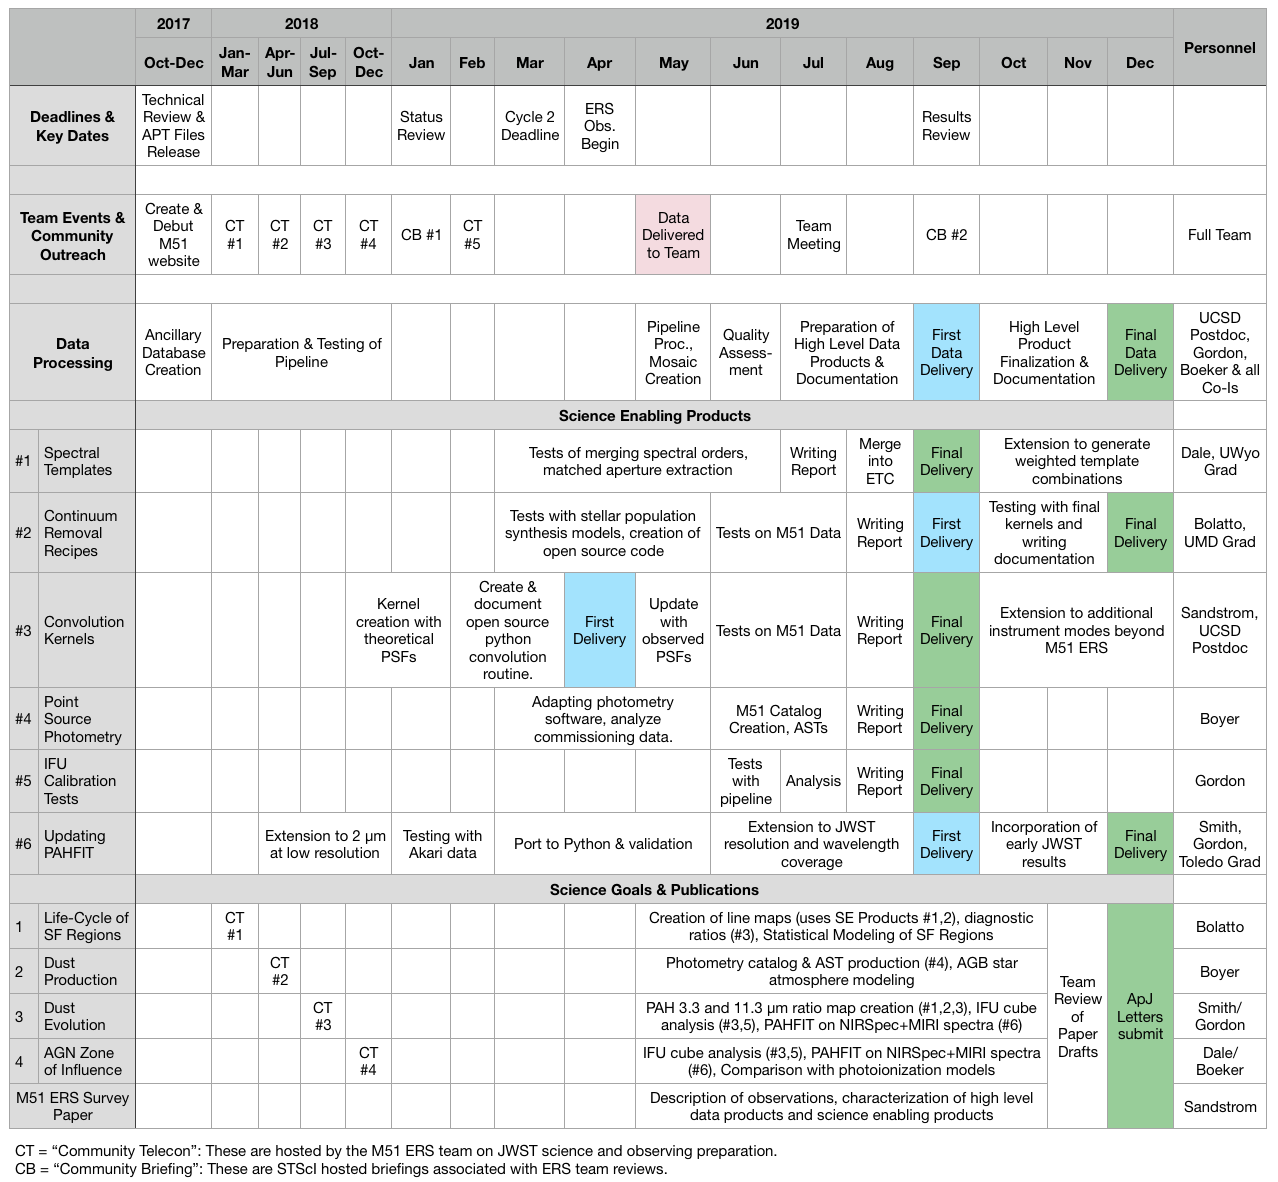
\includegraphics[width=\textwidth]{workplan_crop.png} 
%  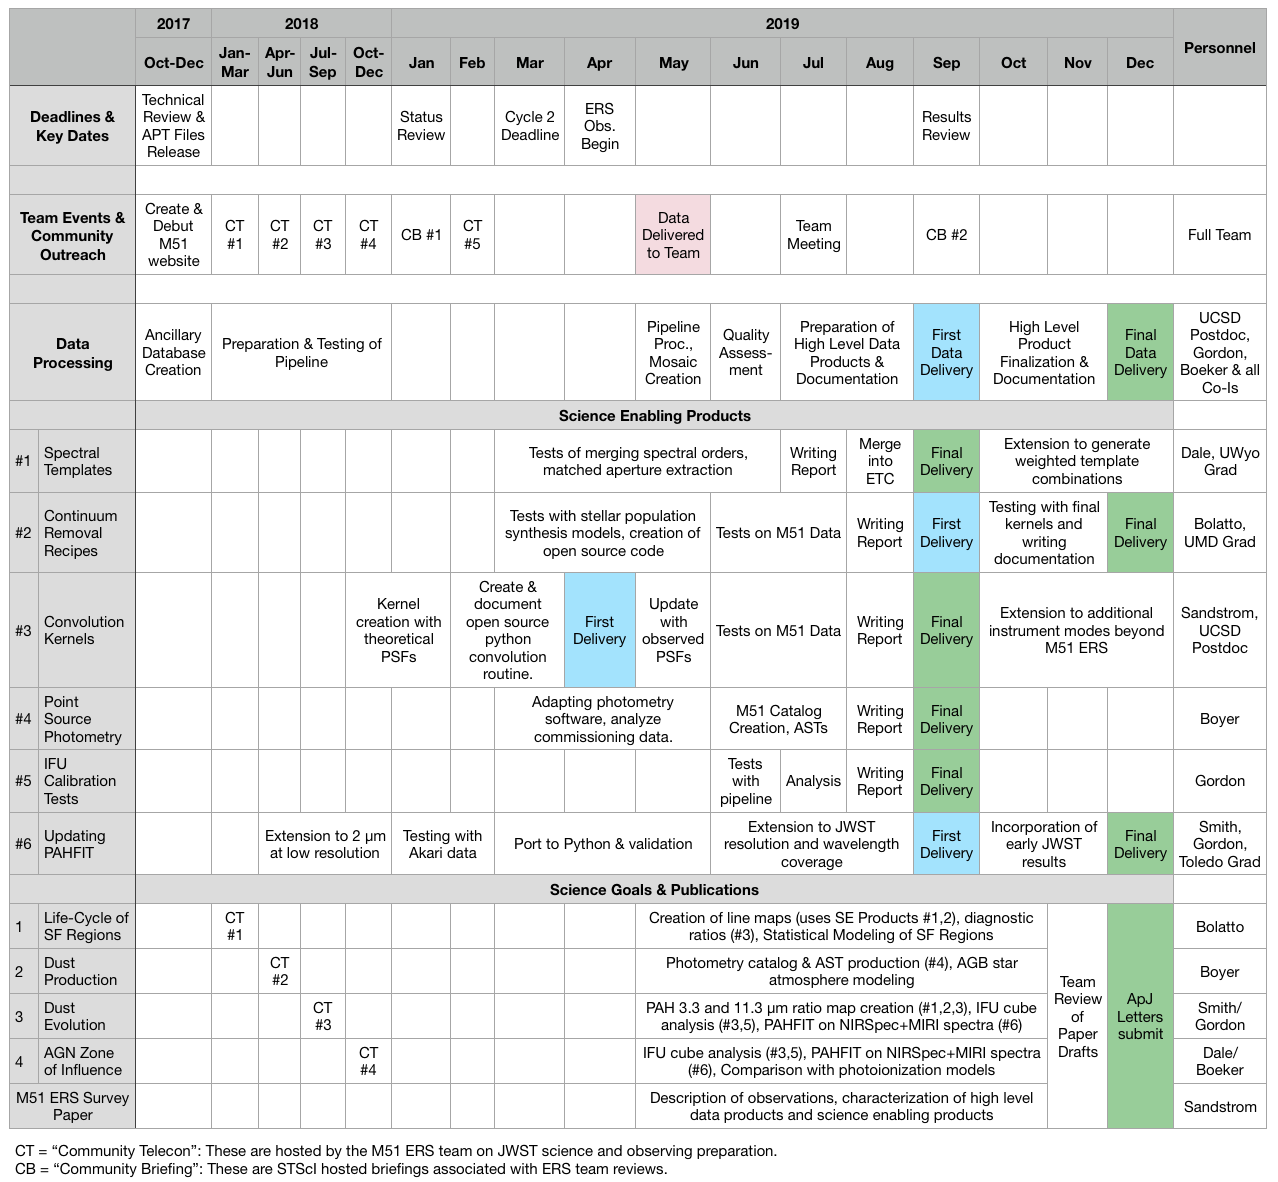
\includegraphics[width=0.9\textwidth]{workplan_crop.png}
%\label{tab:workplan}
%\vspace{-0.3in}
%\end{figure}
%\end{table}
%\end{minipage}

\vspace{-0.1in}
\begin{figure}[h!]
% \plotone{summary_figure}
\begin{center}
Table~4: M51 ERS Work Plan \& Milestones
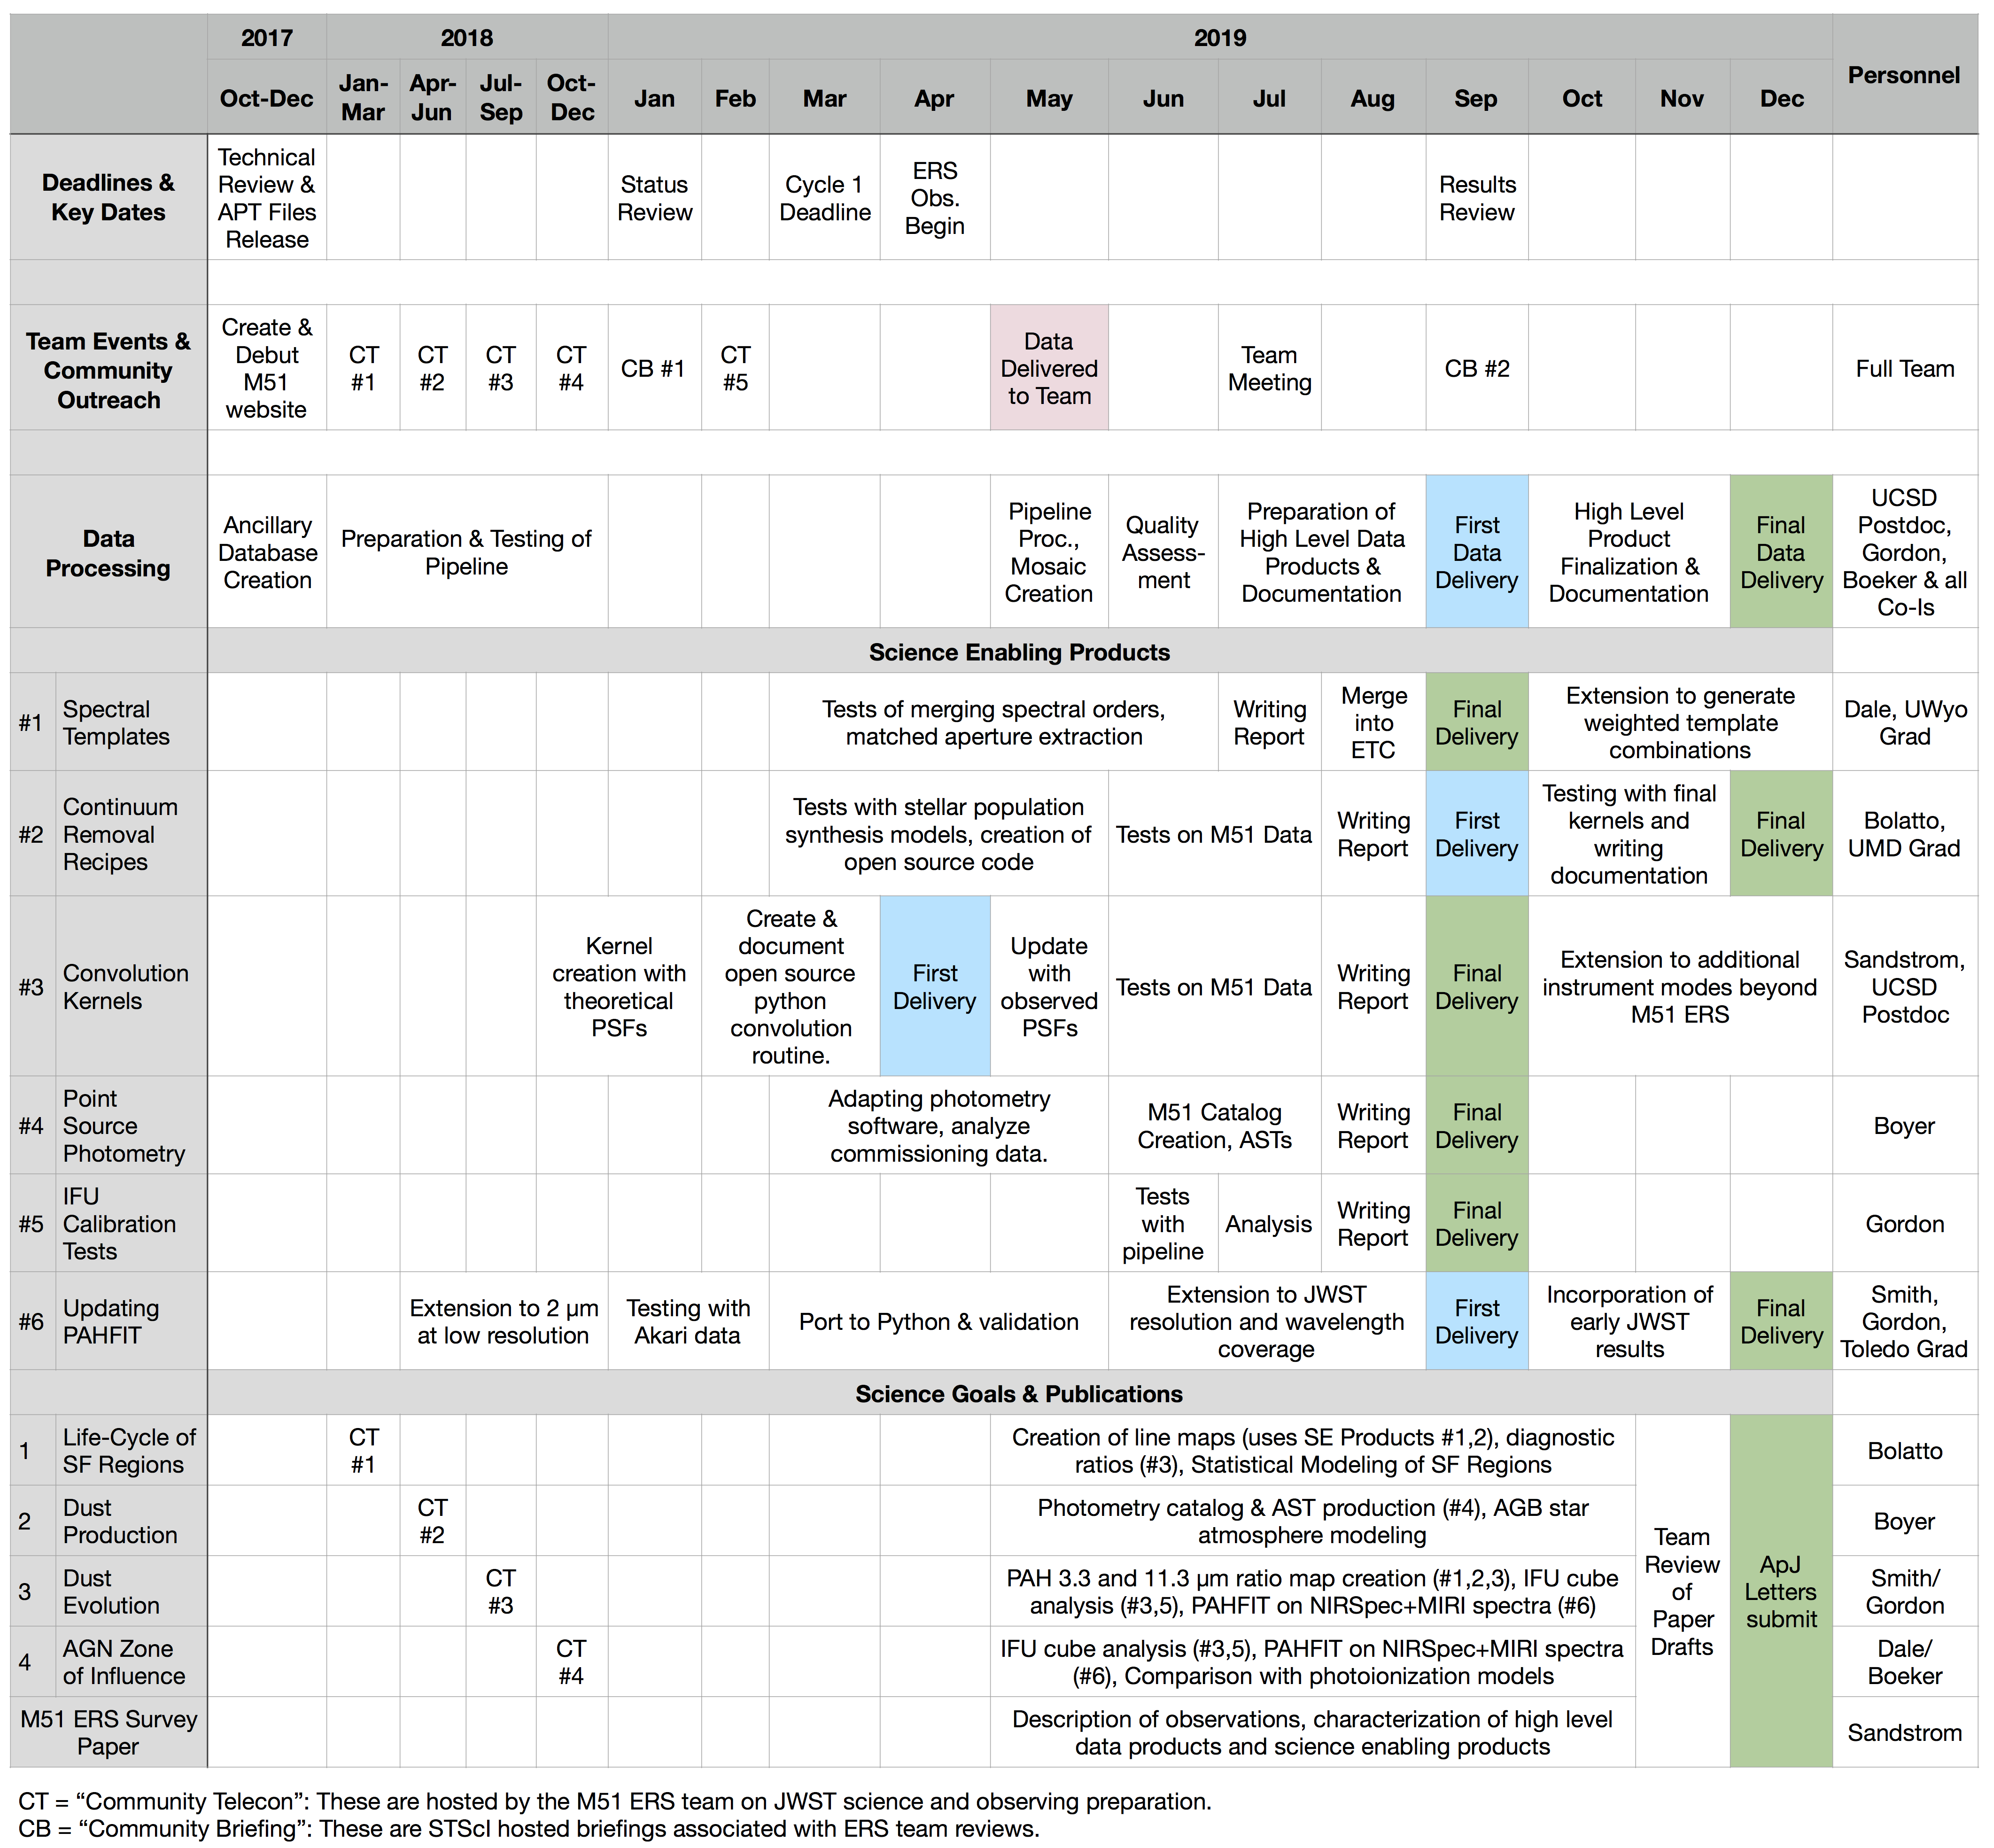
\includegraphics[width=\textwidth]{workplan_crop_new.png} 
%  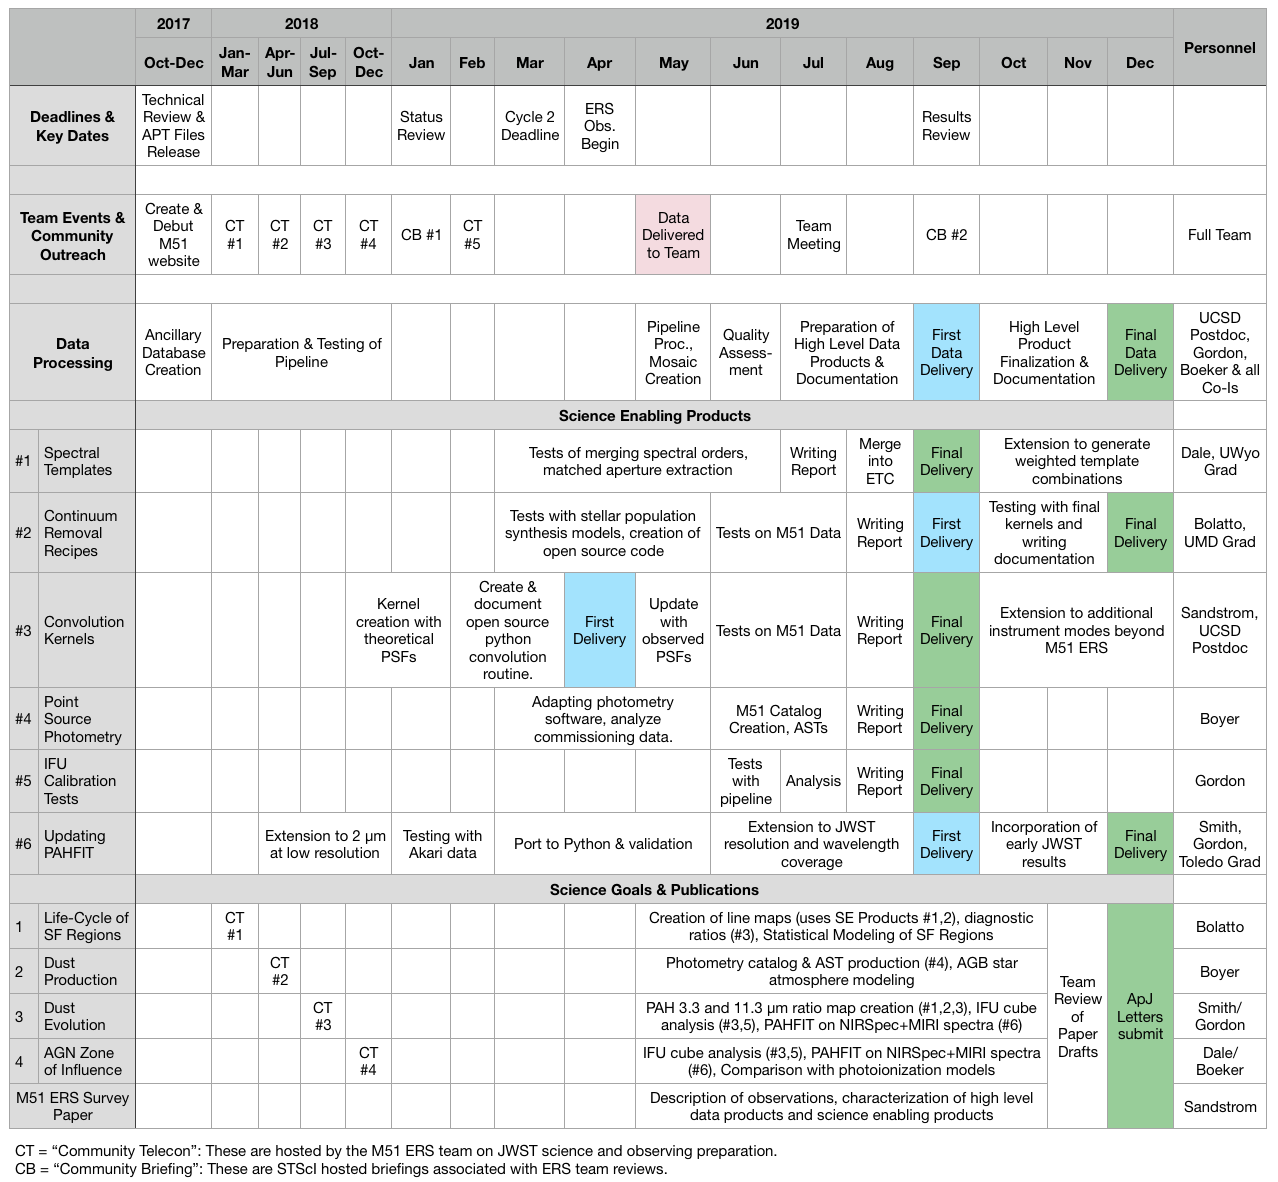
\includegraphics[width=0.9\textwidth]{workplan_crop.png}
\label{tab:workplan}
\vspace{-0.3in}
\end{center}
\end{figure}

%IN PROGRESS The majority of the below science-enabling products will be developed immediately after the data have been taken, nominally during the summer of 2019.  Pre-launch work on PAHFIT and the spectral templates will also be carried out during Summer 2018.

%\vspace{0.1in}

%\noindent {\bf PAHFIT update}: PAHFIT is a popular tool for decomposing mid-infrared spectra of dusty objects and galaxies into their primary components---ionic and molecular lines, warm dust, PAHs, starlight, and  dust attenuation.   Co-I Smith and student will provide an updated version of PAHFIT for the JWST era---JPAHFIT.  Building on the modeling success of PAHFIT for Spitzer/IRS, JPAHFIT will be converted to Python and adapted to the characteristics of JWST spectra  (e.g., ices and CO absorption, new lines and dust features, extended wavelength coverage, various spectral resolutions).  In addition to tuning JPAHFIT by incorporating matched JWST IFU spectra from M51, there will also be pre-launch efforts facilitated by Akari cross-archival training to extend the wavelength coverage down to 2$\micron$. 

%\vspace{0.1in}

%\noindent {\bf Spectral templates}: Co-PI Dale will lead the effort to develop representative $2{-}28\micron$ spectra based on NIRSpec and MIRI IFU data.  The focus will be on H{\small II} regions, nuclear/near-nuclear regions, and arm/inter-arm areas.  The data from the two instruments and their multiple spectral components will be self-consistently normalized and stitched together, with all wavelength gaps bridged, to provide wavelength-complete $2{-}28\micron$ spectra.  

%\vspace{0.1in}

%\noindent {\bf Line maps and narrow band continuum removal recipes}: Co-I Bolatto and student will provide line maps and quantify the effectiveness of empirically-derived recipes for producing them, leveraging the proposed narrow and medium band imaging along with the ``truth'' derived from NIRSpec IFU spectra.  

%\vspace{0.1in}

%\noindent {\bf Point source catalogs}: Co-I Boyer will produce a catalog of the point sources detected in each of the imaging mosaics by adapting existing HST PSF fitting tools for use with JWST.  Right Ascension, Declination, and a preliminary flux and uncertainty will be provided for each object. We will also provide artificial star tests to characterize the photometric completeness and a report outlining how to produce PSF photometry with JWST. 

%\vspace{0.1in}

%\noindent {\bf The utility of LeakCals and spectral ``offs''}: Co-I Gordon will quantify the necessity for taking ``off'' spectra.  He will measure the difference in key spectral map features processed with and without the off spectra, and assess if these differences are significant by comparing to the estimated uncertainties. Likewise, we will measure the importance of taking LeakCal data, including the necessity of taking them for every pointing and whether dithering LeakCal observations improve the final data product.

%\vspace{0.1in}

%\noindent {\bf Convolution kernels}: PI Sandstrom will construct a comprehensive set of smoothing kernels that will enable fair comparisons of JWST data taken at a variety of angular resolutions.  These convolution kernels will be developed for both imaging and spectral data.

%\vspace{0.1in}
%\noindent {\bf Overall Documentation \& Testing:} MIRI MRS pipeline: We will assess the quality of the fringe correction in the pipeline. Impact of the residuals, most affected wavelengths, impact in the SNR of faint emission or absorption lines, whether residuals can be mistaken for lines etc. Just informing the community and giving feedback to the pipeline.

%We will compare the pipeline-produced NIRCam and MIRI mosaics to existing M51 maps from HST and Spitzer, thus providing an early test of the quality of the level 3 data products. If necessary, we will work with STScI to improve the plate scale and/or distortion models used by the JWST pipeline.

%%%%%%%%%%%%%%%%%%%%%%%%%%%%%%%%%%%%%%%%%%%%%%%%%%%%%%%%%%%%%%%%%%%%%%%%%%%


\newpage

\scriptsize
\setlength{\bibsep}{0pt plus 0.3ex}
\bibliography{ers}

\end{document}          % End of proposal. Do not delete this line.
                        % Everything after this command is ignored.